\documentclass[machines,article,submit,moreauthors]{Definitions/mdpi}
\usepackage{tikz}

% MDPI internal metadata commands retained from the supplied template.
\firstpage{1}
\makeatletter
\setcounter{page}{\@firstpage}
\makeatother
\pubvolume{1}
\issuenum{1}
\articlenumber{0}
\pubyear{2026}
\copyrightyear{2026}
\datereceived{}
\daterevised{}
\dateaccepted{}
\datepublished{}

\Title{A Simulation-Based FMU Digital-Twin Workflow for Fault-Informed Thermal Supervisory Control of an Induction Motor}

\newcommand{\orcidauthorA}{0009-0004-2951-7537}
\newcommand{\orcidauthorB}{0000-0001-6189-6478}
\Author{Dilshad Ahmed$^{1,}$\orcidA{}* and Sridhar R$^{2}$\orcidB{}}
\AuthorNames{Dilshad Ahmed and Sridhar R}

\address{%
$^{1}$ \quad Department of Computer Science and Engineering, R.V. College of Engineering (RVCE), Bengaluru, India; dilshadahmed.cs23@rvce.edu.in\\
$^{2}$ \quad Associate Professor, Department of Mechanical Engineering, R.V. College of Engineering (RVCE), Bengaluru, India; sridharr@rvce.edu.in}

\corres{Correspondence: dilshadahmed.cs23@rvce.edu.in}

\abstract{This study presents a simulation-based digital-twin workflow for an 18.5 kW squirrel-cage induction motor composed around the Modelica Standard Library benchmark and exported as a Functional Mock-up Unit (FMU) for Functional Mock-up Interface (FMI) 2.0 Co-Simulation. A Python loop integrates thermal-state estimation, fault diagnosis, 30 s and 60 s temperature forecasting, three supervisory controllers, and an Asset Administration Shell representation. Nominal behavior was checked against the Modelica reference example; the study is not a physical-motor validation. A deterministic campaign covered 11 scenarios and three controllers (33 runs; 2700 s per run; 0.5 s sampling). No run crossed the configured critical policy threshold of 120 degrees C. Scenario-mean maximum winding temperatures were 96.171, 95.343, and 94.825 degrees C for baseline, adaptive, and constrained control, respectively; corresponding mean useful shaft work was 12.377, 13.104, and 13.278 kWh, while electrical energy was 13.639, 14.414, and 14.602 kWh. These deterministic simulation outcomes show policy trade-offs, not statistical generalization or validated protection performance. Thermal parameters and fault magnitudes remain assumptions, and the model has not been validated on physical hardware.}

\keyword{induction motor; digital twin; thermal estimation; fault diagnosis; Modelica; FMU; supervisory control; predictive maintenance}

\begin{document}

\maketitle

\section{Introduction}

This paper documents a simulation-based digital-twin framework for a squirrel-cage induction motor built from the Modelica Standard Library (MSL) machine model and evaluated under a deterministic multi-scenario campaign. The active plant is an 18.5 kW, 400 V, 50 Hz, four-pole induction machine composed around the unmodified MSL squirrel-cage machine component. The project integrates the plant with a lumped winding/frame thermal network, a Functional Mock-up Unit (FMU) exported for Functional Mock-up Interface (FMI) 2.0 Co-Simulation, a Python runtime, a thermal-state estimator, fault diagnosis and severity estimation, 30 s and 60 s forecasting, and supervisory control. The system is not presented as a physical motor-test validation; rather, it is a simulation benchmark for digital-twin experimentation under controlled fault scenarios.

Digital-twin terminology spans models linked to physical assets, model-based digital shadows, and simulation-oriented workflows; these categories are not interchangeable and depend on the direction and timing of data exchange \cite{kritzinger2018}. Induction-motor condition monitoring has a substantial literature on current-signature analysis and comparative fault-diagnosis methods \cite{benbouzid2000,liu2017}. More recent motor-focused digital-twin studies address particular diagnostic settings: Adamou and Alaoui describe efficiency- and loss-based diagnosis for broken-rotor-bar cases, while Chen et al. report a digital-twin method for stator inter-turn short circuits in traction motors \cite{adamou2024,chen2025}. The available publisher metadata and abstracts support these descriptions; full-text methods/results could not be independently reviewed here, so no numerical performance comparison is made. Neither study is treated as a direct controller benchmark for the present work.

The thermal network used here is a lumped engineering approximation; established electric-machine thermal analysis emphasizes that heat paths and boundary conditions matter and that model fidelity depends on the intended application \cite{staton2005}. The present work is therefore an engineering integration and deterministic simulation-evaluation study, not a field-validated industrial deployment or an algorithmic novelty claim. Its bounded contributions are (i) an MSL-based induction-machine FMU linked to an explicit Python estimator/diagnosis/forecast/control loop, (ii) an auditable 11-scenario comparison with true plant values kept separate from Twin estimates, and (iii) a structured six-submodel Asset Administration Shell (AAS) synchronization demonstration. The research questions are: (1) how closely does the composed plant reproduce the MSL nominal operating point under the documented test, and (2) what deterministic trade-offs in thermal outcomes, useful shaft work, energy, and prediction errors are observed across the three implemented controllers? These questions are answerable only for this model and protocol.

The remainder of the paper is organized as follows. Section~\ref{sec:methods} describes the plant model, parameter provenance, thermal network, FMU pipeline, and evaluation protocol. Section~\ref{sec:results} reports the nominal operating-point validation and the 33-run deterministic campaign. Section~\ref{sec:discussion} interprets the results, discusses limitations, and positions the work against prior literature. Section~\ref{sec:conclusions} summarizes the contributions and identifies future validation needs.

\section{Materials and Methods}
\label{sec:methods}

\subsection{System architecture and scope}

The simulated plant composes the unmodified MSL squirrel-cage induction-machine component with a lumped winding/frame thermal network, estimator-facing measurement channels, fault-injection inputs, and supervisory-control interfaces. The model is exported to FMI 2.0 Co-Simulation and executed by a Python runtime that advances the FMU in communication substeps no larger than 0.1 s. True plant variables, estimates, predictions, and controller commands are recorded separately at sample intervals of 0.5 s.

The architecture follows a single closed-loop digital-twin workflow: plant state $\rightarrow$ measurement adaptation $\rightarrow$ thermal estimation $\rightarrow$ fault detection/severity estimation $\rightarrow$ forecast generation $\rightarrow$ controller actuation $\rightarrow$ plant update (Figure~\ref{fig:architecture}). The controller logic is intentionally heterogeneous: baseline control relies on direct thermal condition and threshold logic, whereas adaptive and constrained control also use observer, anomaly, and forecast information. This difference in information access is preserved in the campaign and should be considered when comparing controller outcomes.

The implementation exposes six AAS submodels—OperationalState, ElectricalState, MechanicalState, ThermalState, FaultState, and ControlInterface—following the structured submodel approach in the AAS specification \cite{aas2023}. At each synchronization, a shared snapshot identifier and simulation timestamp are written and read back across the six submodels. This local BaSyx test establishes the tested write/read/alignment behavior only; it is not evidence of an industrial deployment.

\begin{figure}[H]
\centering
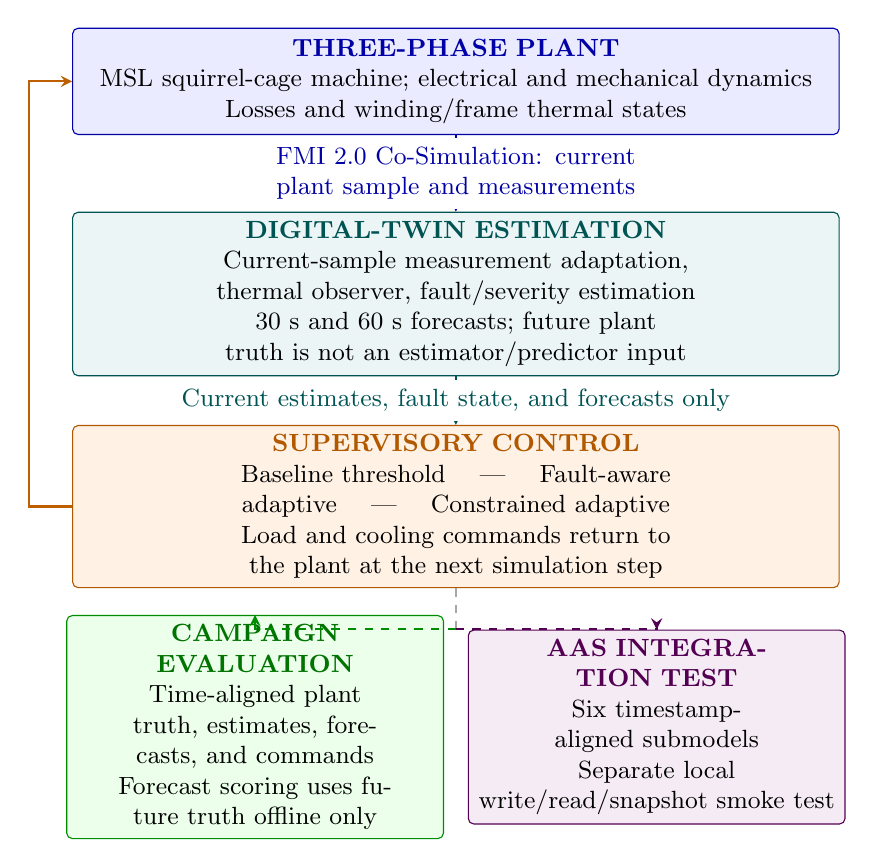
\begin{tikzpicture}[font=\small,>=stealth]
\node[draw=blue!65!black,fill=blue!8,rounded corners=2pt,
      text width=9.5cm,minimum height=1.35cm,align=center] (plant) at (0,0)
  {\textbf{\color{blue!65!black}THREE-PHASE PLANT}\\
   MSL squirrel-cage machine; electrical and mechanical dynamics\\
   Losses and winding/frame thermal states};
\node[draw=teal!65!black,fill=teal!8,rounded corners=2pt,
      text width=9.5cm,minimum height=1.35cm,align=center] (twin) at (0,-2.7)
  {\textbf{\color{teal!65!black}DIGITAL-TWIN ESTIMATION}\\
   Current-sample measurement adaptation, thermal observer, fault/severity estimation\\
   30 s and 60 s forecasts; future plant truth is not an estimator/predictor input};
\node[draw=orange!70!black,fill=orange!10,rounded corners=2pt,
      text width=9.5cm,minimum height=1.35cm,align=center] (control) at (0,-5.4)
  {\textbf{\color{orange!70!black}SUPERVISORY CONTROL}\\
   Baseline threshold \quad | \quad Fault-aware adaptive \quad | \quad Constrained adaptive\\
   Load and cooling commands return to the plant at the next simulation step};
\node[draw=green!55!black,fill=green!8,rounded corners=2pt,
      text width=4.55cm,minimum height=1.2cm,align=center] (evaluation) at (-2.55,-8.2)
  {\textbf{\color{green!45!black}CAMPAIGN EVALUATION}\\
   Time-aligned plant truth, estimates, forecasts, and commands\\
   Forecast scoring uses future truth offline only};
\node[draw=violet!65!black,fill=violet!8,rounded corners=2pt,
      text width=4.55cm,minimum height=1.2cm,align=center] (aas) at (2.55,-8.2)
  {\textbf{\color{violet!65!black}AAS INTEGRATION TEST}\\
   Six timestamp-aligned submodels\\
   Separate local write/read/snapshot smoke test};
\draw[->,thick,blue!65!black] (plant.south) -- node[midway,fill=white,
  text width=8.7cm,align=center] {FMI 2.0 Co-Simulation: current plant sample and measurements}
  (twin.north);
\draw[->,thick,teal!65!black] (twin.south) -- node[midway,fill=white,
  text width=8.7cm,align=center] {Current estimates, fault state, and forecasts only}
  (control.north);
\draw[->,thick,orange!75!black] (control.west) -- ++(-0.55,0) |- (plant.west);
\coordinate (branch) at (0,-6.95);
\draw[thick,dashed,gray!70] (control.south) -- (branch);
\draw[->,thick,dashed,green!55!black] (branch) -| (evaluation.north);
\draw[->,thick,dashed,violet!65!black] (branch) -| (aas.north);
\end{tikzpicture}
\caption{Simulation workflow and evidence paths. Plant truth is recorded separately from Twin estimates; future plant values are used only for post-run forecast scoring and are not estimator or predictor inputs. The Asset Administration Shell (AAS) branch represents a separate local integration test, not a physical deployment.\label{fig:architecture}}
\end{figure}

\subsection{Plant model and parameter provenance}

The selected benchmark is the MSL \texttt{IMC\_withLosses} example in MSL 4.1.0 \cite{msl2024}, which provides a published 18.5 kW, 400 V, 50 Hz, four-pole squirrel-cage induction-machine parameter set and associated nominal operating point. The project does not claim that the benchmark is a manufacturer-identified motor or a field-calibrated machine. Instead, the model is an MSL-based benchmark whose nominal values include rated shaft output, line-to-line RMS voltage, nominal current, efficiency, speed, and loss data.

Table~\ref{tab:parameters} summarizes the model attributes and parameter provenance. Values were obtained from (i) MSL reference data, (ii) literature/reference values, (iii) calculations from documented values and formulas, and (iv) explicit assumptions for thermal and controller configuration. The stator and rotor resistances, leakage inductances, magnetizing inductance, inertia, and loss quantities are inherited from the MSL benchmark or derived from its documented nominal conditions. The winding/frame thermal capacitances and conductances, fault magnitudes, safety thresholds, and controller envelopes are assumptions rather than manufacturer or experimental measurements.

\begin{table}[H]
\caption{Main induction-motor model attributes and provenance. MSL-derived electrical and mechanical values are distinguished from assumed or calculated thermal-network parameters.\label{tab:parameters}}
\begin{tabularx}{\textwidth}{p{0.26\textwidth} p{0.28\textwidth} X}
\toprule
\textbf{Attribute} & \textbf{Value} & \textbf{Provenance} \\
\midrule
Rated shaft output & 18.5 kW & MSL reference data \\
Supply voltage & 400 V line-to-line RMS & MSL reference data \\
Frequency & 50 Hz & MSL reference data \\
Pole count & 4 poles & MSL parameter-record definition \\
Nominal speed & 1462.5 rpm & MSL reference data \\
Nominal efficiency & 90.49\% & MSL reference data \\
Stator and rotor resistances & 0.56 $\Omega$/phase, 0.42 $\Omega$/phase & MSL reference data \\
Magnetizing/leakage inductances & Derived from MSL reactances & Calculated values \\
Rotor inertia & 0.12 kg m$^{2}$ & MSL reference data \\
Ambient temperature & 20 $^{\circ}$C & Explicit assumption \\
Winding heat capacity & 15,000 J K$^{-1}$ & Assumed thermal parameter \\
Frame heat capacity & 35,000 J K$^{-1}$ & Assumed thermal parameter \\
Winding-to-frame resistance & 0.010 K W$^{-1}$ & Assumed thermal parameter \\
Frame-to-ambient resistance & 0.0296652 K W$^{-1}$ & Calculated from MSL loss/reference temperatures and assumed network \\
Winding/fixed loss split & 0.644/0.356 & Calculated from MSL nominal copper and total losses \\
Thermal safety thresholds & 90/100/115/120 $^{\circ}$C policy & Digital-twin configuration \\
\bottomrule
\end{tabularx}
\end{table}

The nominal validation checks the MSL reference operating point rather than a physically instrumented motor. Under balanced nominal three-phase supply, shaft load is ramped to nominal torque and the settled model outputs are compared against the MSL reference values. Voltage, current, frequency, speed, slip, electromagnetic torque, shaft torque, electrical input power, shaft power, efficiency, power factor, and loss components are checked with explicit tolerances. This is a benchmark consistency check, not hardware validation.

\subsection{Thermal model and fault layer}

The plant's winding and frame nodes receive losses from the MSL machine thermal ports. With winding copper loss $P_{\mathrm{w}}$, remaining internal machine loss $P_{\mathrm{f}}$, and effective frame-to-ambient resistance $R_{\mathrm{fa,eff}}$, the implemented two-node balance is
\begin{equation}
C_{\mathrm{w}}\frac{dT_{\mathrm{w}}}{dt}
=P_{\mathrm{w}}-\frac{T_{\mathrm{w}}-T_{\mathrm{f}}}{R_{\mathrm{wf}}},
\qquad
C_{\mathrm{f}}\frac{dT_{\mathrm{f}}}{dt}
=P_{\mathrm{f}}+\frac{T_{\mathrm{w}}-T_{\mathrm{f}}}{R_{\mathrm{wf}}}
-\frac{T_{\mathrm{f}}-T_{\mathrm{a}}}{R_{\mathrm{fa,eff}}}.
\label{eq:plantthermal}
\end{equation}
Here, $C_{\mathrm{w}}=15{,}000$ J K$^{-1}$, $C_{\mathrm{f}}=35{,}000$ J K$^{-1}$, and $R_{\mathrm{wf}}=0.010$ K W$^{-1}$ are assumptions. The nominal frame-to-ambient resistance is 0.0296652 K W$^{-1}$, derived from the selected nominal loss and temperature values under the assumed network. Cooling and thermal-resistance degradation modify effective heat rejection within configured bounds. The model routes winding losses to the winding node and the other MSL thermal-port losses to the frame node; the resulting network does not resolve internal spatial gradients or all physical heat paths. Additional externally imposed friction work is included in the total loss output but is not a separately identified measured thermal input. These dynamics are a model approximation, not a calibrated motor thermal model.

The fault layer applies explicit scenario disturbances to the supply amplitude or frequency, one phase voltage, cooling/thermal resistance, sensor channel, shaft load, or opposing mechanical torque. Table~\ref{tab:scenarios} summarizes the 11 tested scenarios and their modeled mechanisms. Mechanical unbalance and radial vibration are not represented because the plant has no radial mechanical degrees of freedom. Fault amplitudes are stress-test inputs, not calibrated field severities.

\begin{table}[H]
\caption{Deterministic campaign scenarios and the modeled intervention. The mechanisms describe simulation inputs, not validated field fault signatures.\label{tab:scenarios}}
\begin{tabularx}{\textwidth}{l X}
\toprule
\textbf{Scenario} & \textbf{Modeled intervention} \\
\midrule
healthy & No injected fault; nominal reference condition \\
cooling & Reduced frame-to-ambient cooling effectiveness \\
frequency deviation & Supply frequency shifted from nominal \\
mechanical friction & Additional speed-opposing mechanical torque \\
overload & Increased shaft-load torque \\
thermal-resistance degradation & Increased winding-to-frame thermal resistance \\
sensor bias & Additive bias to the winding-temperature sensor channel \\
sensor freeze & Hold the sensor output at its value at fault activation \\
supply degradation & Scale down balanced phase-voltage amplitudes \\
voltage imbalance & Modify one phase voltage to create supply imbalance \\
combined supported & Combined sensor bias, cooling degradation, overload, and supply-voltage reduction \\
\bottomrule
\end{tabularx}
\end{table}

\subsection{FMU runtime, estimation, forecasting, and control}

The FMU runtime advances the exported model using FMI 2.0 Co-Simulation \cite{fmi2020}, converts outputs to the controller interface, and stores true plant channels separately from estimates, forecasts, and commands. The estimator uses current loss/temperature measurements and an internal two-node model; it initializes from the current temperature measurements, propagates winding temperature from the loss balance, and corrects the frame state using its measured innovation. It does not correct the winding estimate directly from the potentially biased/frozen winding sensor. The predictor rolls the same reduced-order model forward in 0.5 s steps to 30 s and 60 s, holding current measured loss inputs and the current cooling command/effectiveness constant over each forecast horizon. Future FMU truth is used only after the run to score the forecasts, not as an estimator/controller input.

The prediction block estimates 30 s and 60 s winding-temperature trajectories from current plant and observer data. The controller block implements a baseline threshold policy, a fault-aware adaptive policy, and a constrained adaptive policy. Table~\ref{tab:controllerinfo} records the respective inputs. The baseline policy uses raw winding-sensor temperature and detector-derived sensor reliability; the adaptive policy uses the state estimate, detector, severity scores, and forecasts; the constrained policy uses estimated and predicted temperatures, overall fault severity, inferred cooling efficiency, and a sensor-reliability factor. Controller signal access is therefore unequal, and the comparison is an engineering trade-off study rather than a matched algorithm benchmark.

The supervisory \texttt{speed\_pu} input scales the supply frequency command within the model; it is not a closed-loop shaft-speed setpoint. The reported shaft speed is an emergent plant output under the electrical supply and load torque. Speed tracking errors are therefore interpreted relative to the nominal V/f reference used by the metric, not as tracking performance of a speed controller.

\begin{table}[H]
\caption{Controller information used by the implemented supervisory policies.\label{tab:controllerinfo}}
\begin{tabularx}{\textwidth}{l X X}
\toprule
\textbf{Controller} & \textbf{Inputs used for its command} & \textbf{Implemented policy} \\
\midrule
Baseline & Raw winding sensor; reliability flag from sensor-bias/freeze detection & Threshold derating at warning/critical temperatures; minimum-load command if sensor is unreliable \\
Adaptive & Estimated winding state; fault detection; severity channels; 30 s and 60 s forecasts & Forecast-/risk-weighted load derating with fault penalties and per-step load-rate limit \\
Constrained & Estimated and forecast winding temperatures; overall fault severity; inferred cooling efficiency; sensor reliability & Prioritizes cooling, then constrained progressive load derating near risk limits \\
\bottomrule
\end{tabularx}
\end{table}

\subsection{Evaluation protocol and reproducibility}

The final deterministic campaign comprises 11 scenarios and three controllers, yielding 33 runs. Each run lasts 2700 s with fault inputs applied from 350 s and 0.5 s control samples. The sample at 350 s is pre-injection; the first faulted sample is at 350.5 s. No stochastic disturbance or random seed is used. Results are computed from raw per-run CSV files and the manifest. Electrical energy is left-endpoint integrated, useful work integrates only positive shaft power, and mean scenario outcomes weight the 11 scenarios equally. Estimation errors compare same-time estimates with FMU truth; forecast errors compare predictions with future truth only during post-run scoring, omitting horizons without a matching future sample. The equations are
\begin{equation}
\begin{aligned}
E_{\mathrm{e}}&=\frac{\sum_i P_{\mathrm{e}}(t_i)\Delta t_i}{3.6\times10^6},\qquad
W_{\mathrm{shaft}}=\frac{\sum_i\max(P_{\mathrm{shaft}}(t_i),0)\Delta t_i}{3.6\times10^6},\\
\mathrm{MAE}_{h}&=\frac{1}{N_h}\sum_{i\in I_h}
\left|\widehat{T}_{\mathrm{w},h}(t_i)-T_{\mathrm{w}}(t_i+h)\right|,
\end{aligned}
\label{eq:metrics}
\end{equation}
where powers are in watts, $\Delta t_i$ is in seconds, energy and work are in kWh, $h\in\{30,60\}$ s, and $I_h$ contains only samples with an aligned target at horizon $h$. The AAS write/read/snapshot smoke test is a separate run. The campaign manifest records Python 3.12.4, Windows 11 (build 22621), NumPy 2.5.3, pandas 3.0.6, FMPy 0.3.32, and Matplotlib 3.11.2. OpenModelica 1.27.1 and MSL 4.1.0 were used for FMU export and nominal validation; detailed hardware model/RAM information was not recorded. The campaign manifest records base commit \texttt{d14c35ff2e73ebf743c970f7585b3c3030140b97} and a non-clean working tree. The source and configuration changes recorded in that working-tree status have since been committed and pushed at \url{https://github.com/Dilshad-Ahmed1/Industrial-Motor-DT/commit/74a5fb3015bb9055cb81499e7676e1479d003104}; hashes of the campaign Modelica source and primary Twin configuration match the manifest. From the repository root, the documented campaign and artifact-regeneration commands are:
\begin{verbatim}
.\.venv\Scripts\python.exe -m experiments.run_research_evaluation
.\.venv\Scripts\python.exe -m experiments.run_research_evaluation `
  --with-basyx
.\.venv\Scripts\python.exe -m analysis.generate_research_artifacts `
  --campaign results\research_evaluation\<UTC timestamp>
\end{verbatim}
For the separate local AAS smoke test, the documented service launch and seed commands are:
\begin{verbatim}
docker compose -f docker\docker-compose.yml up -d
.\.venv\Scripts\python.exe scripts\seed_basyx.py
\end{verbatim}
The optional \texttt{--with-basyx} campaign mode is separate from the completed AAS smoke-test evidence. No random seed or stochastic input is used.

\section{Results}
\label{sec:results}

\subsection{Nominal validation}

The nominal validation step compares the model against the benchmark MSL reference operating point for a balanced 400 V, 50 Hz, nominal-load condition. All explicit tolerance checks passed under OpenModelica 1.27.1 and MSL 4.1.0. Table~\ref{tab:validation} reports the observed settled values and signed deviation (simulation minus reference) for the primary operating-point variables. The run demonstrates nominal consistency with the MSL benchmark point, not independent physical validation of an identified motor.

\begin{table}[H]
\caption{Nominal operating-point check against the MSL reference. Deviations are simulation output minus reference; the validation JSON reports that each measure passed its configured tolerance.\label{tab:validation}}
\begin{tabularx}{\textwidth}{l r r r}
\toprule
\textbf{Quantity} & \textbf{Reference} & \textbf{Simulation} & \textbf{Deviation} \\
\midrule
Line voltage (V) & 400.000 & 400.000 & $<0.001$ \\
Line current (A) & 32.850 & 32.857 & +0.0065 \\
Supply frequency (Hz) & 50.000 & 50.000 & 0.000 \\
Shaft speed (rpm) & 1462.500 & 1462.894 & +0.394 \\
Slip (\%) & 2.500 & 2.474 & $-0.026$ percentage points \\
Electromagnetic torque (N m) & 122.637 & 122.638 & +0.0009 \\
Shaft torque (N m) & 120.795 & 120.795 & $<0.0001$ \\
Electrical input power (kW) & 20.444 & 20.444 & +0.00036 \\
Shaft output power (kW) & 18.500 & 18.505 & +0.00498 \\
Efficiency (\%) & 90.490 & 90.514 & +0.024 percentage points \\
Power factor & 0.8980 & 0.8981 & +0.00011 \\
Total motor losses (W) & 1943.950 & 1939.330 & $-4.620$ \\
\bottomrule
\end{tabularx}
\end{table}

\subsection{Deterministic campaign overview}

The final campaign executed 33 completed runs, with no failed runs. Raw traces, a campaign manifest, and summary metrics provide the underlying evidence. Table~\ref{tab:campaign} reports the mean values across the equally weighted scenario set for the three controllers. These are deterministic scenario averages, not statistical estimates of population-level motor performance or field behavior.

\begin{table}[H]
\caption{Mean deterministic campaign values over the 11 equally weighted scenarios for each controller. Values should be interpreted as scenario-level averages rather than statistical estimates.\label{tab:campaign}}
\begin{tabularx}{\textwidth}{l c c c}
\toprule
\textbf{Metric} & \textbf{Baseline} & \textbf{Adaptive} & \textbf{Constrained} \\
\midrule
Mean maximum winding temperature & 96.171 $^{\circ}$C & 95.343 $^{\circ}$C & 94.825 $^{\circ}$C \\
Mean useful shaft work & 12.377 kWh & 13.104 kWh & 13.278 kWh \\
Mean electrical energy & 13.639 kWh & 14.414 kWh & 14.602 kWh \\
Mean winding-estimation MAE & 1.131 $^{\circ}$C & 0.943 $^{\circ}$C & 1.036 $^{\circ}$C \\
30 s forecast MAE & 0.934 $^{\circ}$C & 0.721 $^{\circ}$C & 0.819 $^{\circ}$C \\
60 s forecast MAE & 1.022 $^{\circ}$C & 0.764 $^{\circ}$C & 0.869 $^{\circ}$C \\
\bottomrule
\end{tabularx}
\end{table}

Figure~\ref{fig:temperature} shows representative winding-temperature trajectories and illustrates that no configured run exceeded the 120 $^{\circ}$C critical threshold. The smallest minimum thermal safety margin was 7.259 $^{\circ}$C in the baseline cooling-degradation case, in which the maximum winding temperature reached 112.741 $^{\circ}$C. This result confirms only that the simulated traces remained below the configured threshold; it does not validate a manufacturer-specific thermal limit or motor protection boundary.

\begin{figure}[H]
\centering
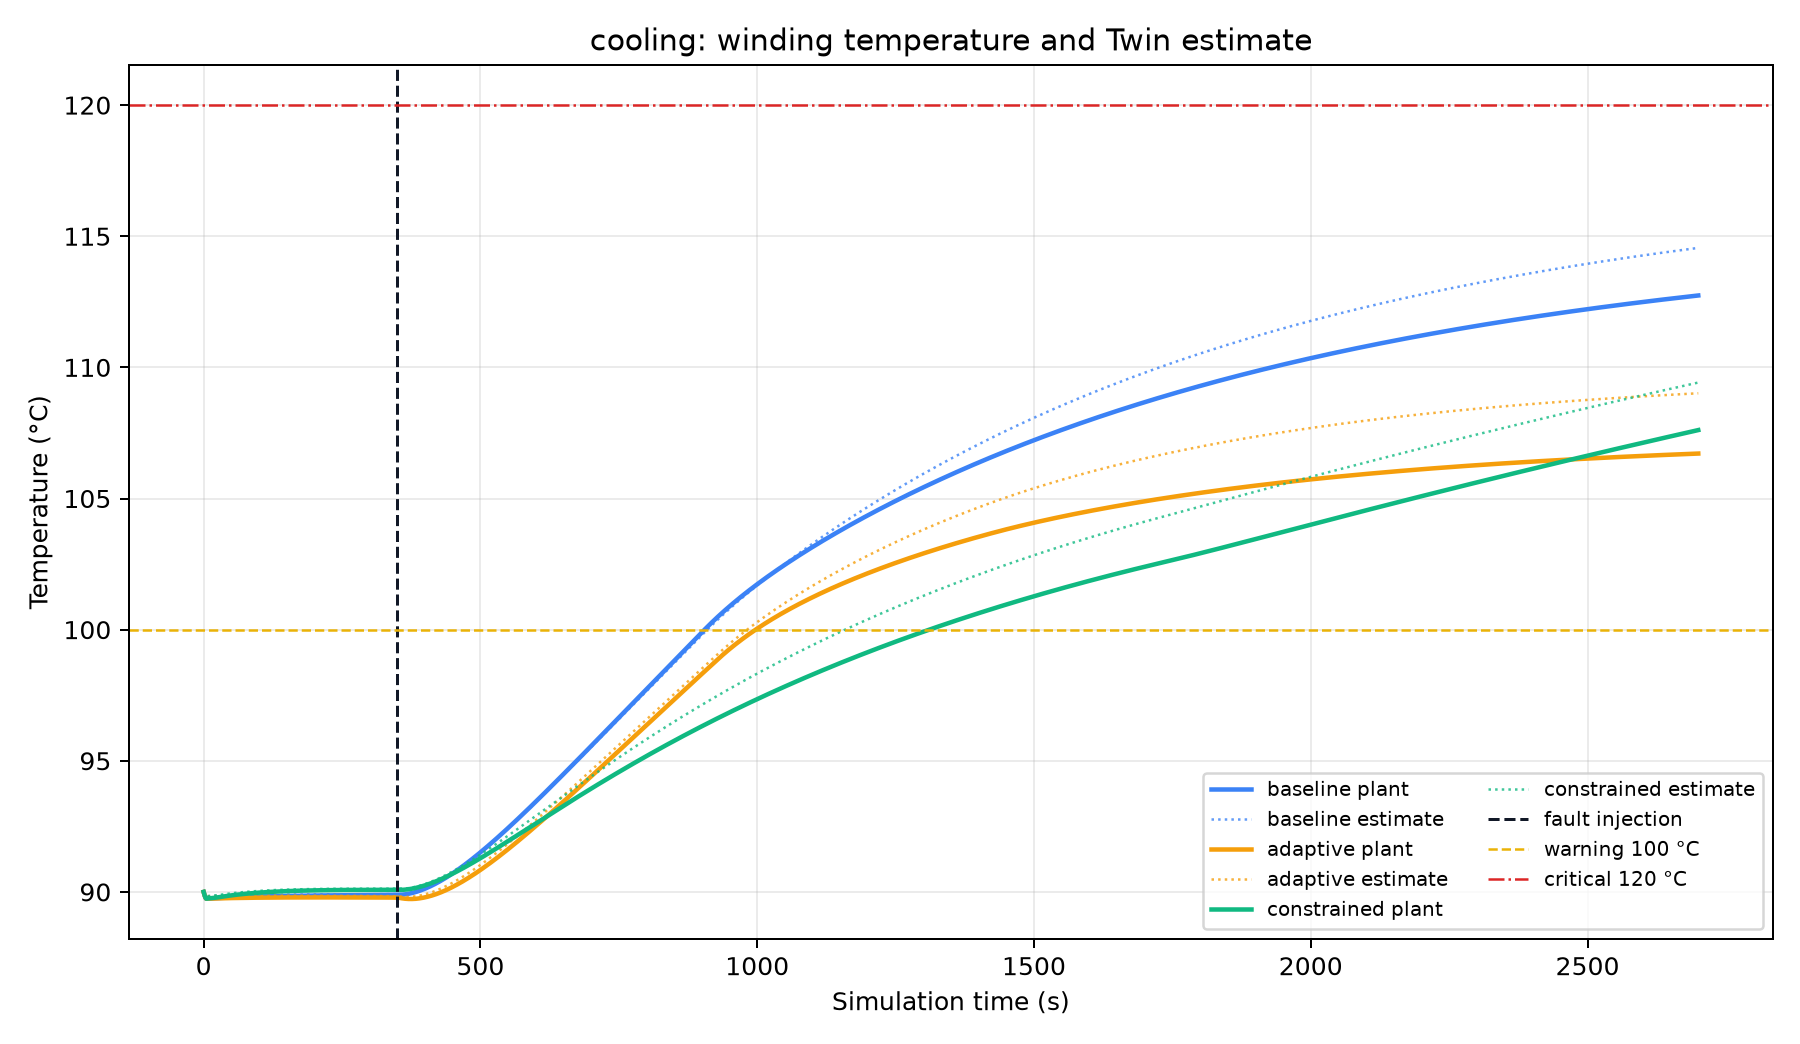
\includegraphics[width=0.92\textwidth]{figures/temperature_cooling.png}
\caption{Winding-temperature truth and Twin estimates for the cooling-degradation scenario for all three controllers. Fault input is applied at 350 s; the sample at 350 s is pre-fault and the first faulted sample is at 350.5 s. The 100 $^{\circ}$C warning and 120 $^{\circ}$C critical lines are configured policy thresholds, not validated motor safety limits.\label{fig:temperature}}
\end{figure}

Figure~\ref{fig:voltageimbalance} shows the winding-temperature response and Twin estimates for voltage imbalance. It provides a second fault case in which controller behavior and estimator-to-plant differences can be inspected directly; it does not establish physical diagnostic accuracy.

\begin{figure}[H]
\centering
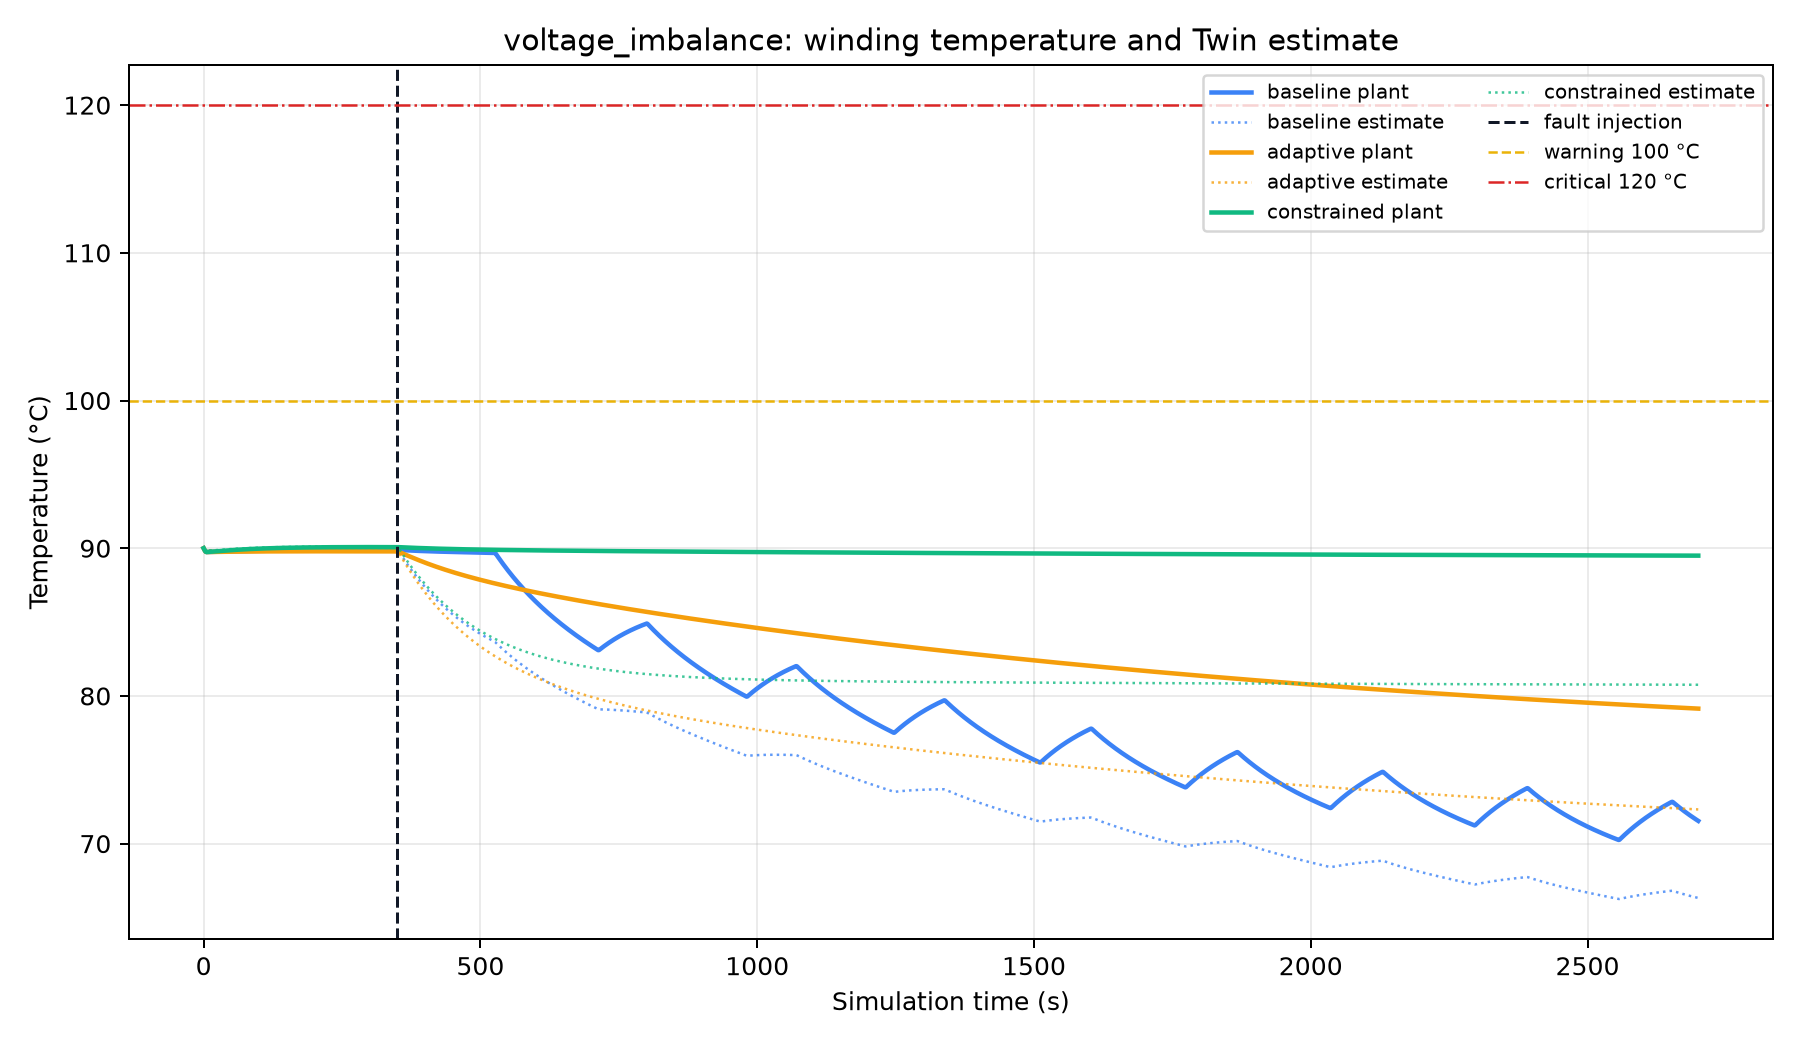
\includegraphics[width=0.92\textwidth]{figures/temperature_voltage_imbalance.png}
\caption{Winding-temperature plant truth and Twin estimates for the voltage-imbalance scenario. The fault input is applied at 350 s; the 100 $^{\circ}$C and 120 $^{\circ}$C lines denote configured warning and critical policy thresholds, not validated motor safety limits. The discrepancy among plant and estimate trajectories illustrates this simulated case only.\label{fig:voltageimbalance}}
\end{figure}

Figure~\ref{fig:loadcommand} compares the three supervisory load commands in the cooling-degradation scenario. The commands diverge after fault activation because the policies use different measurements and estimated/predicted information, as summarized in Table~\ref{tab:controllerinfo}.

\begin{figure}[H]
\centering
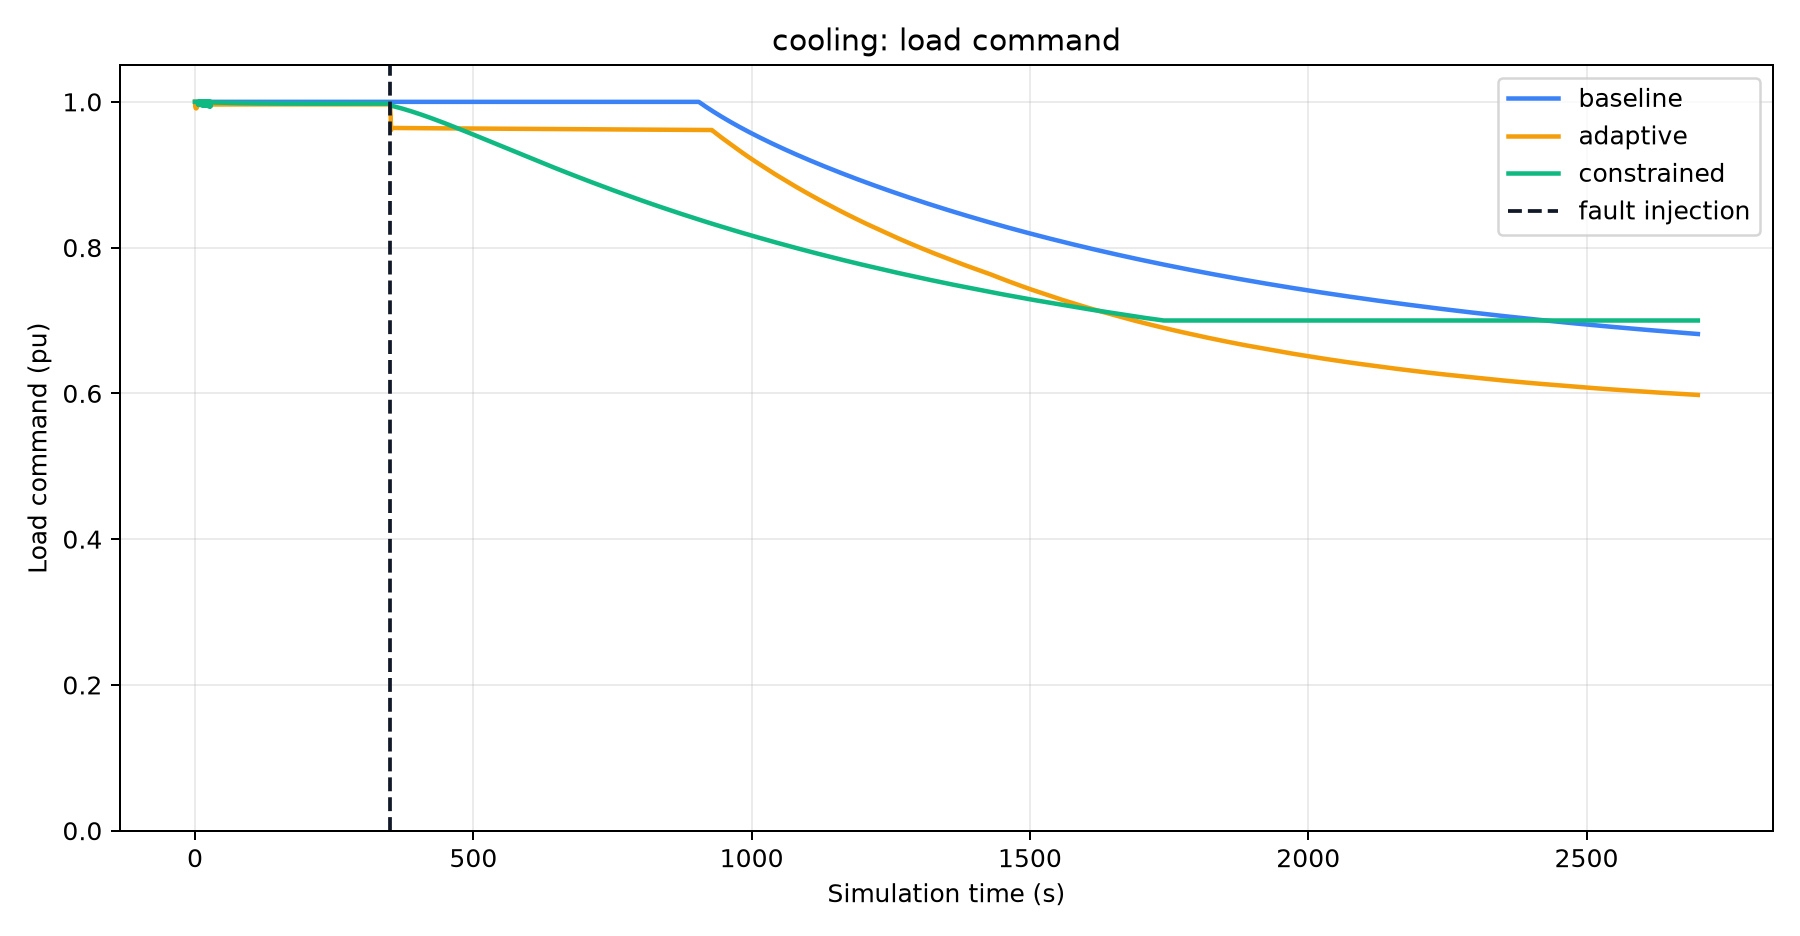
\includegraphics[width=0.92\textwidth]{figures/load_command_cooling.png}
\caption{Normalized load command during the cooling-degradation scenario for the baseline, adaptive, and constrained policies. The vertical dashed line marks fault injection at 350 s. This trace documents the implemented commands in one deterministic run and is not evidence of a generally optimal control response.\label{fig:loadcommand}}
\end{figure}

\subsection{Estimation and forecasting performance}

Winding-estimation mean absolute error (MAE) and 30 s/60 s forecast MAE were evaluated for each controller. On the deterministic scenario-average basis, adaptive control has the lowest average forecast MAE; constrained control has the lowest mean maximum winding temperature and the highest mean useful shaft work, together with higher electrical energy than baseline. These outcomes are not a universal ranking: the controllers use different information and policies, and each scenario/controller pair is one deterministic run. Figure~\ref{fig:forecast} presents scenario-level forecast error and illustrates substantial variation among the tested scenarios.

\begin{figure}[H]
\centering
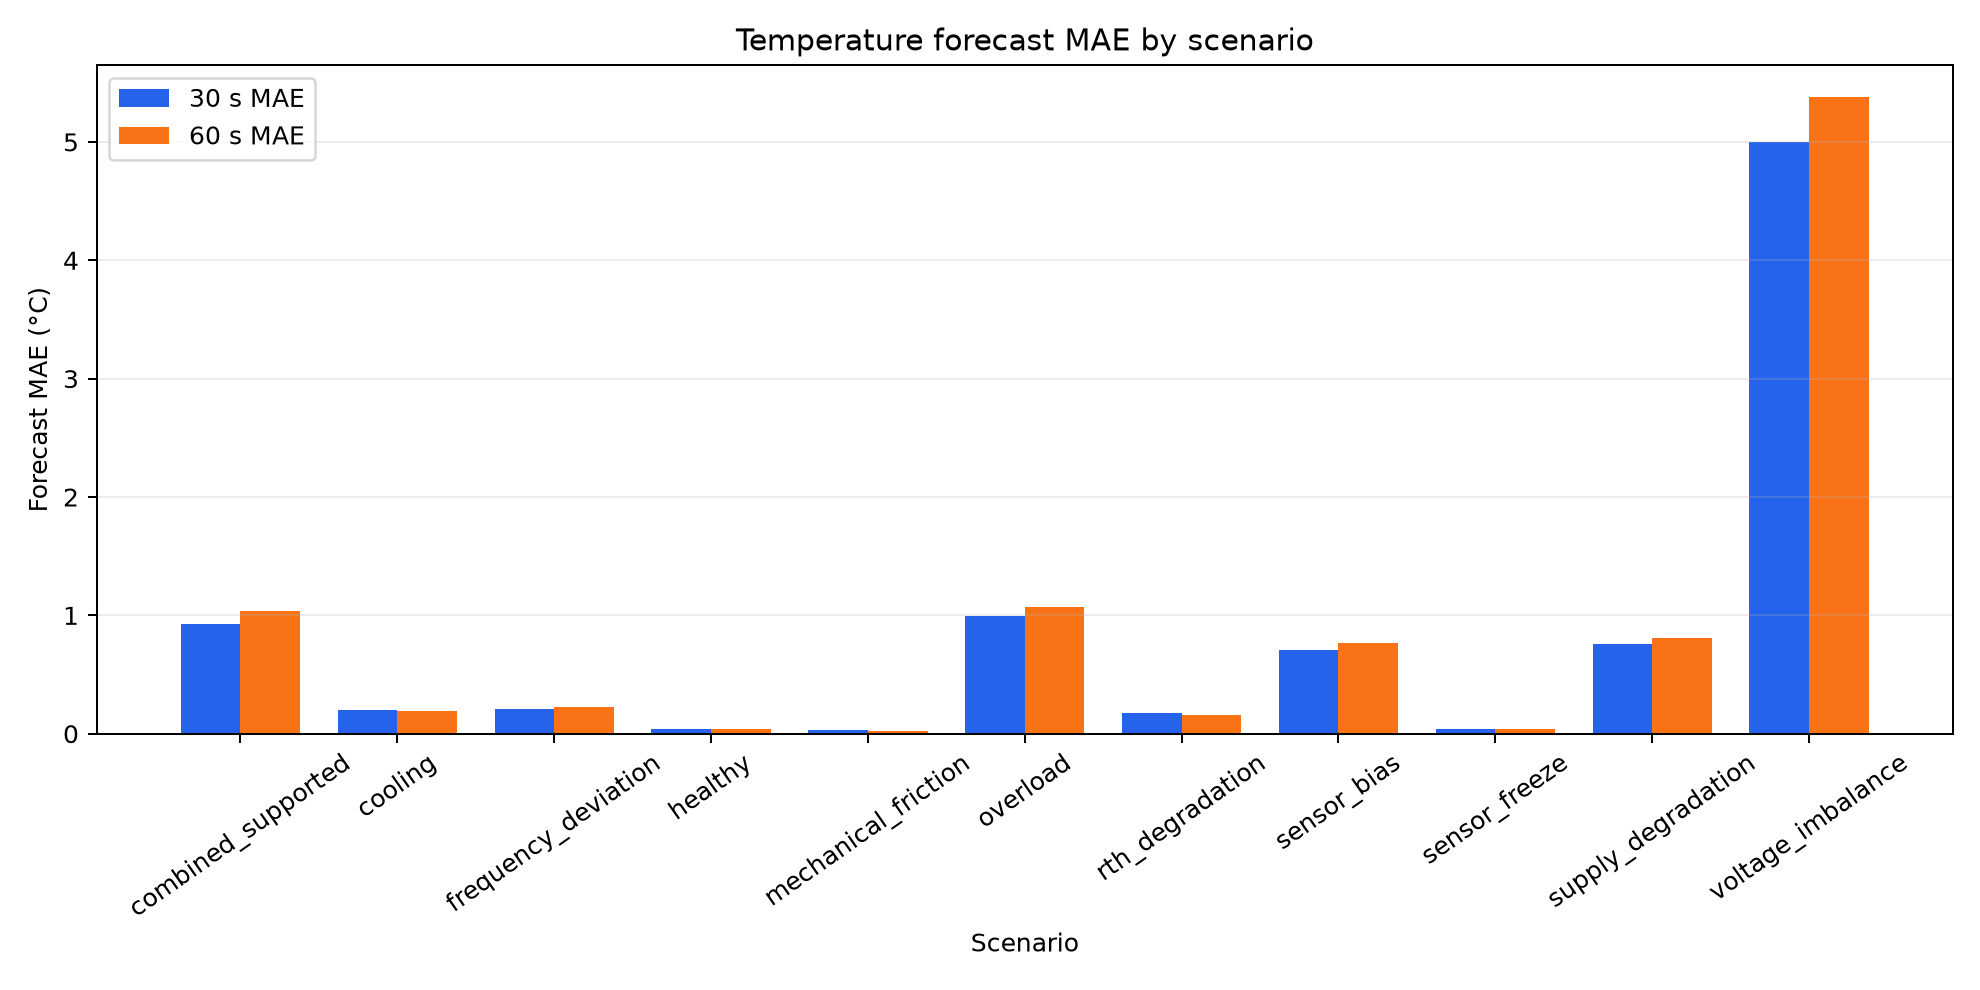
\includegraphics[width=0.92\textwidth]{figures/prediction_mae.png}
\caption{Temperature forecast mean absolute error by scenario at 30 s and 60 s. Values are deterministic scenario-level errors computed from aligned future truth samples; they are not repeated-run uncertainty estimates. The voltage-imbalance case has substantially larger errors than the other tested cases.\label{fig:forecast}}
\end{figure}

\subsection{BaSyx smoke test}

The live BaSyx AAS workflow was evaluated separately from the main deterministic campaign. The smoke test recorded one successful write, 12 successful reads, and one aligned snapshot across the six named submodels. The measured end-to-end synchronization loop took 1055.599 ms and write latency was 443.361 ms; mean read latency was 50.623 ms with a reported p95 of 133.255 ms across the observed reads. The single write and single snapshot are not a statistically meaningful latency distribution. These values demonstrate local write/read/snapshot behavior only, not a real-time guarantee or industrial deployment.

\section{Discussion}
\label{sec:discussion}

This study provides an engineering integration contribution, not a claim of physical motor certification. The FMU-based workflow demonstrates an end-to-end digital-twin pipeline with an MSL induction-machine benchmark. The implemented workflow connects Modelica plant modeling to co-simulation, observer/forecast logic, scenario-based fault injection, and deterministic controller comparison. It also demonstrates how AAS submodel semantics can be integrated into a digital-twin loop. These contributions should not be overstated as proven field performance or industrial deployment.

Prior work establishes that induction-motor diagnosis spans current-signature methods, fault-specific digital-twin models, and thermal-analysis approaches \cite{benbouzid2000,liu2017,adamou2024,chen2025,staton2005}. This project does not claim a new diagnosis or control algorithm and does not compare against those studies' diagnostic benchmarks. Its contribution is an implementation/evaluation artifact: a composed MSL machine with explicit thermal and fault interfaces, a Python loop that separates current Twin estimates from simulation truth, and a deterministic report of thermal, energy, useful-work, and prediction outcomes. The MSL benchmark is not an identified commercial motor, the thermal network is assumption-based, and fault severities are synthetic scenario inputs rather than measured industrial degradation.

The results also reveal several fundamental limitations. The plant is an MSL example-based model, not a manufacturer-identified or physically calibrated motor. Thermal capacitances and resistances are assumed or calculated from assumed network structure; the two-node network aggregates core and other machine losses and omits detailed thermal paths and spatial gradients. External degradation-friction work is not separately coupled as heat to the network. Fault magnitudes, residual thresholds, and 100/120 $^{\circ}$C warning/critical values are not validated against equipment. Residual thresholds were tuned using simulated channels, and the model does not reproduce measured sensor noise/dynamics. Mechanical unbalance and radial vibration are not modeled. Finally, the 33 runs are deterministic single runs with no stochastic replication, so the results do not estimate uncertainty or real-motor generalization.

The controller comparison is also only partially comparable because the system does not give all controllers identical signal access. The baseline controller uses a more limited set of thermal and operating indicators, while the adaptive and constrained controllers additionally exploit observer and forecast outputs. Therefore, the results should be read as an engineering trade-off study rather than as a universal statement that one controller is superior. The adaptive controller shows the best average forecast accuracy and strong thermal safety, while the constrained controller is competitive on useful work and thermal safety, but no universal ranking should be inferred beyond the tested deterministic scenarios.

\section{Conclusions}
\label{sec:conclusions}

This manuscript documents a simulation-based digital-twin workflow for an MSL-based induction motor with thermal-state estimation, simulated fault diagnosis, forecasting, and supervisory control. The evidence supports three bounded conclusions: the composed 18.5 kW model is nominally consistent with the selected MSL reference point under the stated test; the final deterministic campaign has no simulated trace at or above the configured 120 $^{\circ}$C threshold; and the three policies produce distinct scenario-average outcomes in thermal temperature, useful shaft work, electrical energy, and forecast error. None of these results establishes physical fault-detection performance, manufacturer-specific safety, real-time capability, or industrial deployment.

The project does not claim field validation, manufacturer calibration, real-time certification, or general industrial deployment. The work is better described as a transparent and reproducible simulation-based digital-twin engineering framework with explicit limitations and clearly separated evaluation evidence. Future work should prioritize plant-level experimental calibration, measured thermal parameter identification, updated diagnostic thresholds from physical data, and broader validation studies that compare digital-twin estimates against instrumented motor tests.

\authorcontributions{Software, investigation, and writing---original draft preparation, D.A.; supervision and writing---review and editing, S.R. The corresponding author reports that both authors reviewed the prior draft and agreed to submission after the requested revisions; the authors should confirm approval of this revised version before submission.}

\funding{This research received no external funding.}

\institutionalreview{Not applicable. This study used numerical simulation and did not involve human participants or animals.}

\informedconsent{Not applicable.}

\dataavailability{The source and configuration for the evaluated workflow are available at the versioned project commit \url{https://github.com/Dilshad-Ahmed1/Industrial-Motor-DT/commit/74a5fb3015bb9055cb81499e7676e1479d003104}. The campaign manifest identifies the earlier base commit and a non-clean working tree; the source changes recorded in that status were subsequently committed at the linked revision, and the Modelica source and primary Twin configuration hashes match the manifest.}

\supplementary{No supplementary files are currently deposited. The linked source commit provides the evaluated source and configuration; the raw campaign traces are not included in the public repository.}

\acknowledgments{During manuscript preparation, the authors used GitHub Copilot in Visual Studio Code (version information was not available in the project environment) to assist with literature/source discovery, organization of evidence, and manuscript drafting. The authors reviewed and edited the manuscript and are responsible for verifying the accuracy and integrity of all AI-assisted content, citations, numerical values, and interpretations before submission. The authors also acknowledge the Modelica Association and the FMI community for the simulation standards and tools used in this work.}

\conflictsofinterest{The authors declare no conflicts of interest.}

\begin{thebibliography}{99}
\bibitem{kritzinger2018} Kritzinger, W.; Karner, M.; Traar, G.; Henjes, J.; Sihn, W. Digital Twin in Manufacturing: A Categorical Literature Review and Classification. \emph{IFAC-PapersOnLine} \textbf{2018}, 51(11), 1016--1022. \url{https://doi.org/10.1016/j.ifacol.2018.08.474}.

\bibitem{benbouzid2000} Benbouzid, M.E.H. A Review of Induction Motors Signature Analysis as a Medium for Faults Detection. \emph{IEEE Transactions on Industrial Electronics} \textbf{2000}, 47(5), 984--993. \url{https://doi.org/10.1109/41.873206}.

\bibitem{liu2017} Liu, Y.; Bazzi, A.M. A Review and Comparison of Fault Detection and Diagnosis Methods for Squirrel-Cage Induction Motors: State of the Art. \emph{ISA Transactions} \textbf{2017}, 70, 400--409. \url{https://doi.org/10.1016/j.isatra.2017.06.001}.

\bibitem{adamou2024} Adamou, A.A.; Alaoui, C. Efficiency-Centered Fault Diagnosis of In-Service Induction Motors for Digital Twin Applications: A Case Study on Broken Rotor Bars. \emph{Machines} \textbf{2024}, 12(9), 604. \url{https://doi.org/10.3390/machines12090604}.

\bibitem{chen2025} Chen, Y.; Zhao, L.; Li, L.; Liu, K.; Ye, C. Digital Twin-Based Online Diagnosis Method for Inter-Turn Short Circuit Fault in Stator Windings of Induction Motors. \emph{Energies} \textbf{2025}, 18(12), 3063. \url{https://doi.org/10.3390/en18123063}.

\bibitem{staton2005} Staton, D.; Boglietti, A.; Cavagnino, A. Solving the More Difficult Aspects of Electric Motor Thermal Analysis in Small and Medium Size Industrial Induction Motors. \emph{IEEE Transactions on Energy Conversion} \textbf{2005}, 20(3), 620--628. \url{https://doi.org/10.1109/TEC.2005.847979}.

\bibitem{msl2024} Modelica Association. \emph{Modelica Standard Library, Version 4.1.0}; Modelica Association: Linköping, Sweden, 2024. Available online: \url{https://github.com/modelica/ModelicaStandardLibrary/releases/tag/v4.1.0} (accessed on 18 October 2026).

\bibitem{fmi2020} Modelica Association. \emph{Functional Mock-Up Interface (FMI) for Model Exchange and Co-Simulation, Version 2.0}. Available online: \url{https://fmi-standard.org/} (accessed on 18 October 2026).

\bibitem{aas2023} Industrial Digital Twin Association. \emph{Specification of the Asset Administration Shell: Part 1—Metamodel}; IDTA 01001-3-0, Version 3.0.1. Available online: \url{https://industrialdigitaltwin.org/en/content-hub/aasspecifications} (accessed on 18 October 2026).
\end{thebibliography}

\end{document}
